\section{Архитектура и используемые технические средства}

%\subsection{Микросервисная архитектура приложения}
%Микросервисная архитектура — распространенный подход к разработке программного обеспечения, когда приложение разбивается на небольшие автономные компоненты (микросервисы) с четко определенными интерфейсами. Именно эта архитектура характерна для cloud-native приложений, которые сейчас популярны благодаря преимуществам, что открывают для бизнеса облачные среды.
%
%\begin{figure}[h]
%	\centering
%	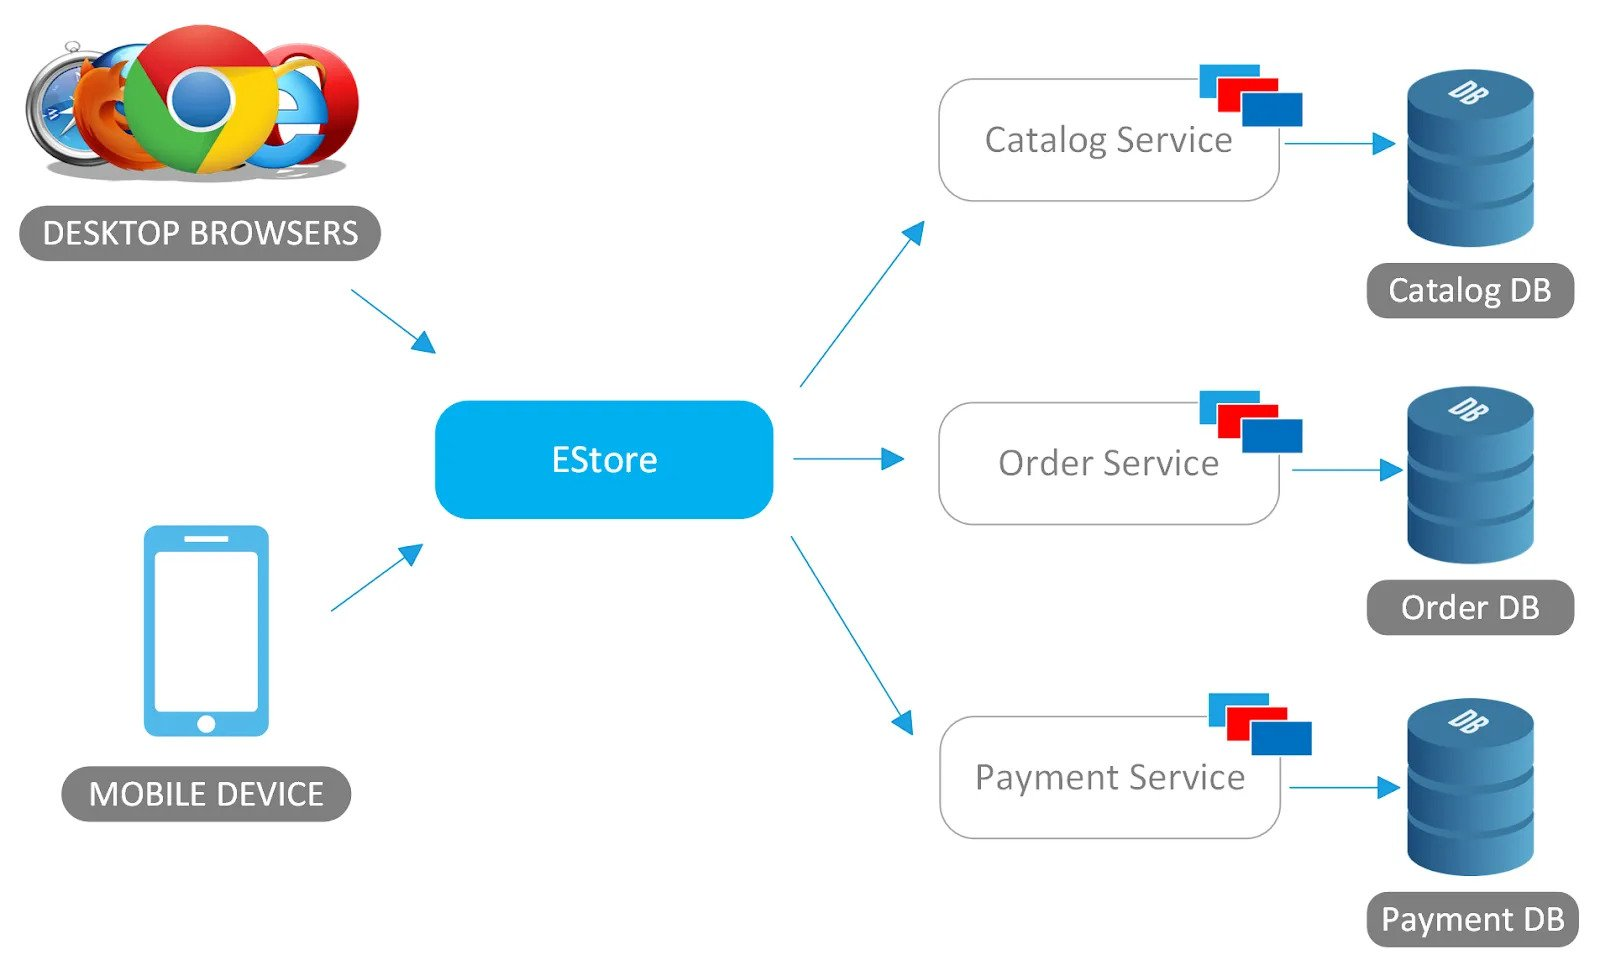
\includegraphics[width=0.7\textwidth]{microservices}
%	\caption{Пример микросервисной архитектуры.}
%	\label{fig:microservices}
%\end{figure}
%{\color{red} TODO https://mcs.mail.ru/blog/prostym-jazykom-o-mikroservisnoj-arhitekture }
%
%К преимуществам такой архитектуры можно отнести следующие факторы:
%\begin{itemize}
%	\item Можно развертывать только изменяющиеся микросервисы, независимо от остальной системы, что позволяет производить обновления чаще и быстрее.
%	\item Можно расширять только те сервисы, которые в этом нуждаются, то есть сервисы с наименьшей производительностью, оставляя работать остальные части системы на менее мощном оборудовании.
%	\item Отказ одного сервиса не приводит к остановке системы в целом. Когда же ошибка исправлена, необходимое изменение можно развернуть только для соответствующего сервиса — вместо повторного развертывания всего приложения. Правда, для этого еще на этапе проектирования микросервисов потребуется тщательно продумать связи между ними для достижения максимальной независимости друг от друга, а также заложить возможность корректного оповещения пользователя о временной недоступности определенного сервиса без ущерба для всей системы.
%	\item Можно подбирать различные наборы технологий, оптимальные для решения задач, стоящих перед отдельными сервисами.
%	\item Присутствует возможность повторного использования функциональности для различных целей и различными способами.
%	\item Небольшие сервисы проще заменить на более подходящую версию или удалить вовсе — это несет значительно меньше рисков по сравнению с монолитным приложением.
%\end{itemize}
%
%\subsection{TypeScript}
%TypeScript — это язык программирования, в котором исправлены многие недостатки JavaScript. Код на TypeScript выглядит почти так же, как и код на JS, и, если у вас есть опыт frontend-разработки, изучить TypeScript достаточно просто. Особенно учитывая, что вы можете писать JS-код прямо в TS-скриптах.
%
%Код на TypeScript компилируется в JS и подходит для разработки любых проектов под любые браузеры — тем более что можно выбрать версию JS, в которую будет компилироваться код.
%
%TypeScript — проект с открытым исходным кодом, поэтому он очень быстро развивается. Многое, что появляется в TS, позже переходит и в JavaScript: например, let и const, стрелочные функции и так далее.
%
%В TypeScript типизация статическая, что избавляет от множества проблем. Есть числовой тип, строковый, логический и другие.
%
%И в JS, и в TS есть поддержка объектно-ориентированного программирования: классы, объекты, наследование. Однако TypeScript шагнул чуть дальше и использует больше возможностей ООП.
%
%\subsection{React Native}
%
%Кроссплатформенная разработка приложений позволяет разработчикам создавать мобильные приложения для нескольких операционных систем одновременно. Проще говоря, эти приложения будут совместимы как с Android, так и с iOS. Он предоставляет разработчикам возможность создавать приложения на базе одного кода и разворачивать их на всех других платформах, что позволяет выпускать программное обеспечение/продукт намного быстрее и качественнее. Кроме того, такой продукт получается более безопасным.
%
%React Native это библиотека JavaScript, которая используется для разработки приложений для систем iOSи Android.
%
%React Native отличный инструмент для разработки сложных кросс-платформенных приложений. Если вы планируете масштабный и популярный продукт, подумайте о том, чтобы использовать React Native. Он имеет обширную документацию и сильную техподдержку. Кроме того, стоит выбирать React Native, если вы планируете повторно использовать код для настольного приложения и WEB-приложения.
%
%Принципы работы React Native практически идентичен ReactJS, кроме того, что React Nativeне управляет DOM через Virtual DOM. Он непосредственно работает в фоновом режиме на устройстве пользователя, что объясняет JavaScript, написанный разработчиками.
%
%Кроме того, он взаимодействует с собственным устройством через сериализацию, пакетный мост и облегчает асинхронную связь. React Native не использует HTML. Он использует чистый JavaScript с синтаксисом JSX.
%
%{
%	\color{red}
%Two years after the 2015 ReactJS release, Facebook created React Native. While the ReactJS library is developed for creating web interfaces, React Native is a hybrid app-development framework for iOS and Android that allows you to reuse up to 95 percent of code leaving the rest to designing platform-specific interfaces.
%
%React and React Native: what the difference? All technical differences between them are caused by platform aims.
%
%While ReactJS uses Virtual DOM to render browser code, React Native uses native APIs as a bridge to render components on mobile. For example, for Android components, it uses Java APIs and it invokes Objective-C API to render to iOS.
%React Native doesn’t use HTML. So, if you worked with ReactJS before, you’ll have to get familiar with React Native syntax. For example, it uses <Text> instead of <p> and <View> instead of <div>.
%Because React Native doesn’t use CSS, standard CSS-features like animation run with React Native special APIs.
%
%The working principles of React Native are virtually identical to React except that React Native does not manipulate the DOM via the Virtual DOM. It runs in a background process (which interprets the JavaScript written by the developers) directly on the end-device and communicates with the native platform via serialized data over an asynchronous and batched bridge.[16][17][18]
%
%React components wrap existing native code and interact with native APIs via React’s declarative UI paradigm and JavaScript. This enables native app development for whole new teams of developers, and can let existing native teams work much faster.[19]
%
%While React Native styling has a similar syntax to CSS, it does not use HTML or CSS.[20] Instead, messages from the JavaScript thread are used to manipulate native views. React Native also allows developers to write native code in languages such as Java or Kotlin for Android and Objective-C or Swift for iOS, which makes it even more flexible.
%}

